\section{Apresentar possíveis parceiros}

\par Esta funcionalidade apresenta ao usuário possíveis parceiros que poderão compor a sua rede de relacionamentos. Para realizar esta busca, também foi preciso escrever uma consulta que levasse em conta dois níveis de análise, sendo elas, a busca pelo possível parceiro dentro da empresa onde o usuário trabalha, levando em conta a quantidade de parceiros em comum entre ambos (usuário autenticado e o possível parceiro) e a busca por parceiros dentro da mesma cidade, também seguindo este mesmo critério. O Código~\ref{list:consulta_possiveis_parceiros} apresenta a \textit{query} utilizada para realizar esta busca.

\begin{lstlisting} [style=custom_SQL,caption={[\textit{Query} para apresentar possíveis parceiros]{\textit{Query} para apresentar possíveis parceiros. \textbf{Fonte:} Elaborado pelos autores.}}, label=list:consulta_possiveis_parceiros] 	
MATCH (me:Person {email: 'andressa_faria18@hotmal.com'}), (users:Person),
(users)-[:WORKS_IN]->(company)<-[:WORKS_IN]-(me)
WHERE users <> me AND users.typeOfAccount <> 'SERVICE_PROVIDER'
AND NOT((users)-[:PARTNER_OF]->(me)-[:PARTNER_OF]->(users)) 
OPTIONAL MATCH
	pMutualFriends=(me)-[:PARTNER_OF]->(another)-[:PARTNER_OF]->(me),
	(users)-[:PARTNER_OF]->(another)-[:PARTNER_OF]->(users)
RETURN DISTINCT({name: users.name, email: users.email, length: 1, 
photo: users.photo, qtde: count(DISTINCT pMutualFriends)}) as person
ORDER BY person.length, person.qtde DESC
UNION ALL
MATCH (me:Person {email: 'andressa_faria18@hotmal.com'}), (users:Person),
(users)-[:LIVES_IN]->(city)<-[:LIVES_IN]-(me)
WHERE NOT((users)-[:WORKS_IN]->()<-[:WORKS_IN]-(me))
AND users.typeOfAccount <> 'SERVICE_PROVIDER'
AND NOT((users)-[:PARTNER_OF]->(me)-[:PARTNER_OF]->(users))
OPTIONAL MATCH 
	pMutualFriends=(me)-[:PARTNER_OF]->(another)-[:PARTNER_OF]->(me),
	(users)-[:PARTNER_OF]->(another)-[:PARTNER_OF]->(users)
RETURN DISTINCT({name: users.name, email: users.email, length: 2, 
photo: users.photo, qtde: count(DISTINCT pMutualFriends)}) as person
ORDER BY person.length, person.qtde DESC
\end{lstlisting}

% Trocado de figura para listagem
%\newpage
%\begin{figure}[h!]
%	\centerline{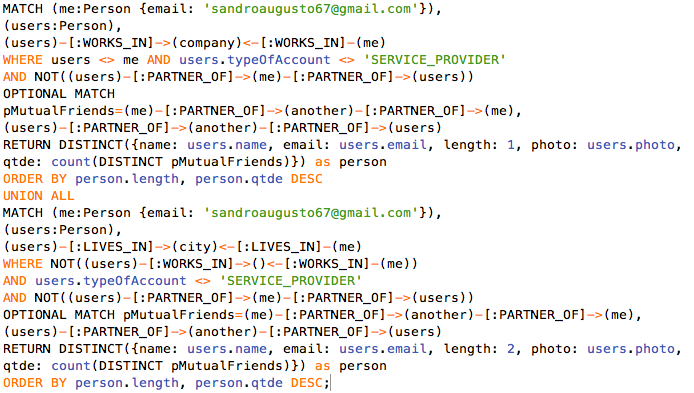
\includegraphics[scale=0.6]{./imagens/consulta-busca-possiveis-parceiros.png}}
%	\caption[\textit{Query} para apresentar possíveis parceiros.]
%	{\textit{Query} para apresentar possíveis parceiros \textbf{Fonte:} Elaborado pelos autores.}
%	\label{fig:consulta_possiveis_parceiros}
%\end{figure}

Essa consulta é dividida em duas sub consultas separadas pela cláusula \texttt{UNION ALL}, a fim de atingir um número maior de possíveis parceiros ao usuário, sendo que a primeira delas está recuperando os dados de pessoas que trabalham na empresa cujo o usuário autenticado no sistema trabalha e não possua o relacionamento de ''parceria'' com ele. A última sub consulta é responsável por obter os dados de pessoas que vivem na cidade cujo o usuário autenticado vive, porém não possuem relacionamento de ''parceria'' e não trabalham na mesma empresa.

\par A Figura~\ref{fig:busca_possiveis_parceiros} apresenta o resultado da busca por possíveis parceiros, contendo uma lista com as pessoas que atendam os requisitos pré estabelecidos na consulta.

\begin{figure}[h!]
	\centerline{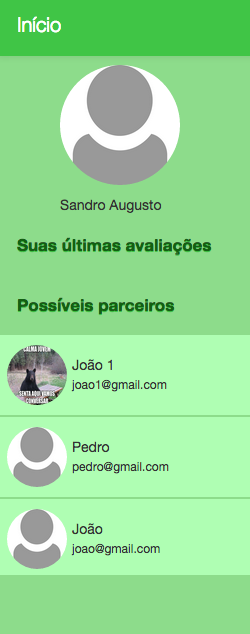
\includegraphics[scale=0.4]{./imagens/busca-possiveis-parceiros.png}}
	\caption[\textit Funcionalidade que apresenta a lista com possíveis parceiros]
	{\textit Funcionalidade que apresenta a lista com possíveis parceiros \textbf{Fonte:} Elaborado pelos autores.}
	\label{fig:busca_possiveis_parceiros}
\end{figure}

\par A ideia desta funcionalidade foi apresentar um possível parceiro que provavelmente já tenha algum vínculo com o usuário ou que possua afinidade com alguém da sua rede de parceria.